\documentclass[12pt]{article} % use larger type; default would be 10pt
\usepackage[utf8]{inputenc} % set input encoding (not needed with XeLaTeX)

%%% PAGE DIMENSIONS
\usepackage{geometry} % to change the page dimensions
\geometry{a4paper} % or letterpaper (US) or a5paper or....
\geometry{margin=2cm} % or letterpaper (US) or a5paper or....

\usepackage{graphicx} % support the \includegraphics command and options
\usepackage[parfill]{parskip} % Activate to begin paragraphs with an empty line rather than an indent
\usepackage{times} % for Times Roman default font

%%% PACKAGES
\usepackage{booktabs} % for much better looking tables
\usepackage{array} % for better arrays (eg matrices) in maths
\usepackage{paralist} % very flexible & customisable lists (eg. enumerate/itemize, etc.)
\usepackage{verbatim} % adds environment for commenting out blocks of text & for better verbatim
\usepackage{subfig} % make it possible to include more than one captioned figure/table in a single float

%%% HEADERS & FOOTERS
\usepackage{fancyhdr} % This should be set AFTER setting up the page geometry
\pagestyle{fancy} % options: empty , plain , fancy
\renewcommand{\headrulewidth}{0pt} % customise the layout...
\lhead{}\chead{}\rhead{}
\lfoot{}\cfoot{\thepage}\rfoot{}

\makeatletter
\renewcommand{\maketitle}{%
  {\bfseries{\scshape{\Large{\@title\par}}}}
}
\makeatother

\hyphenation{Kiwi-bank} % otherwise it may get hyphenated as Ki-wibank

%%% END Article customizations

%%% The "real" document content comes below...

\title{Mt Norma Route: 28 June 2017}

\begin{document}
  \maketitle

When we walked into Lucretia Biv in May we noticed a DoC sign indicating a route to Mt Norma.  I subsequently read that the NZ Deer Stalkers Association had taken on maintining this track (and the route to the Sylvia Tops which we have yet to explore).  So this trip was a recce of the route.

It was in as a good a shape as I had hoped (and better than I expected) and very easy to follow.  The gradient up the ridge is not steep (for this area) and we arrived at the bushline about 1$\frac{1}{2}$ hours after leaving the car (at Palmer Lodge).  A further half hour or so took us to our lunch spot just beyond point 1532.  After lunch we returned to the car which took one hour twenty.

\begin{figure}[ht]
%\centering
\begin{minipage}{.5\linewidth}
\begin{flushleft}
   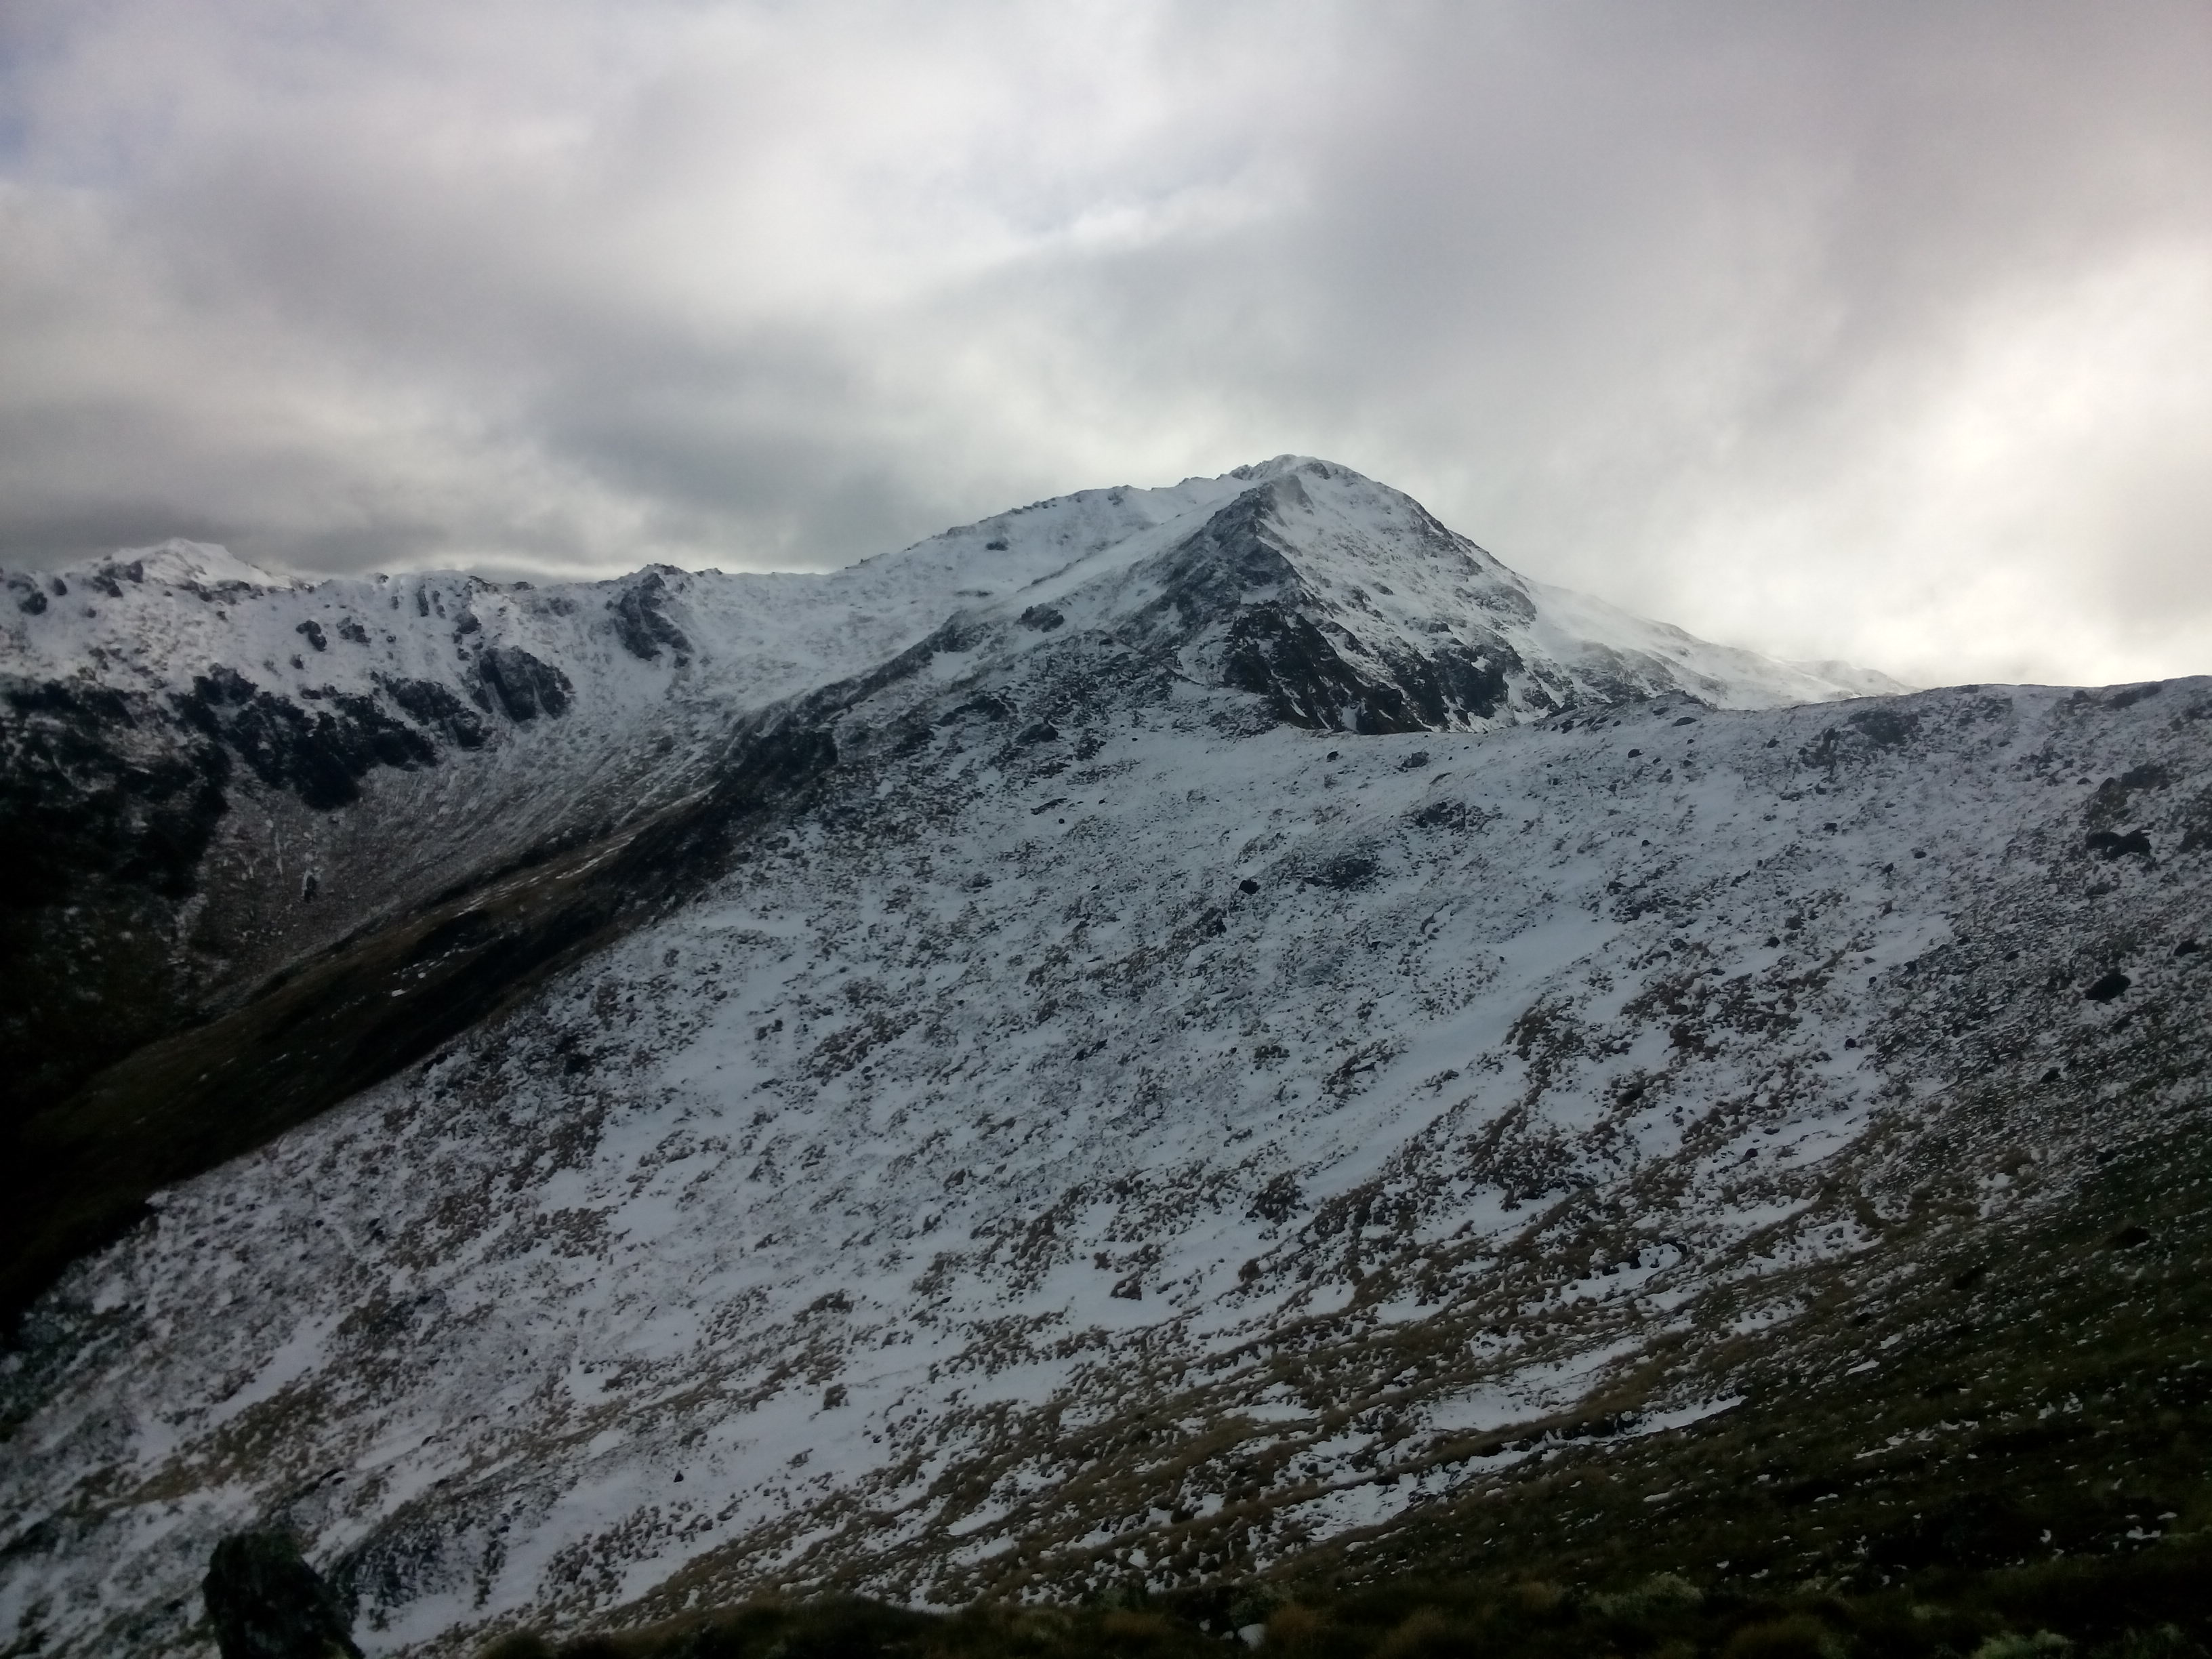
\includegraphics[width=8.5cm]{MtNorma28June2017Photo1}
\end{flushleft}
\end{minipage}
\begin{minipage}{.5\linewidth}
\begin{flushright}
    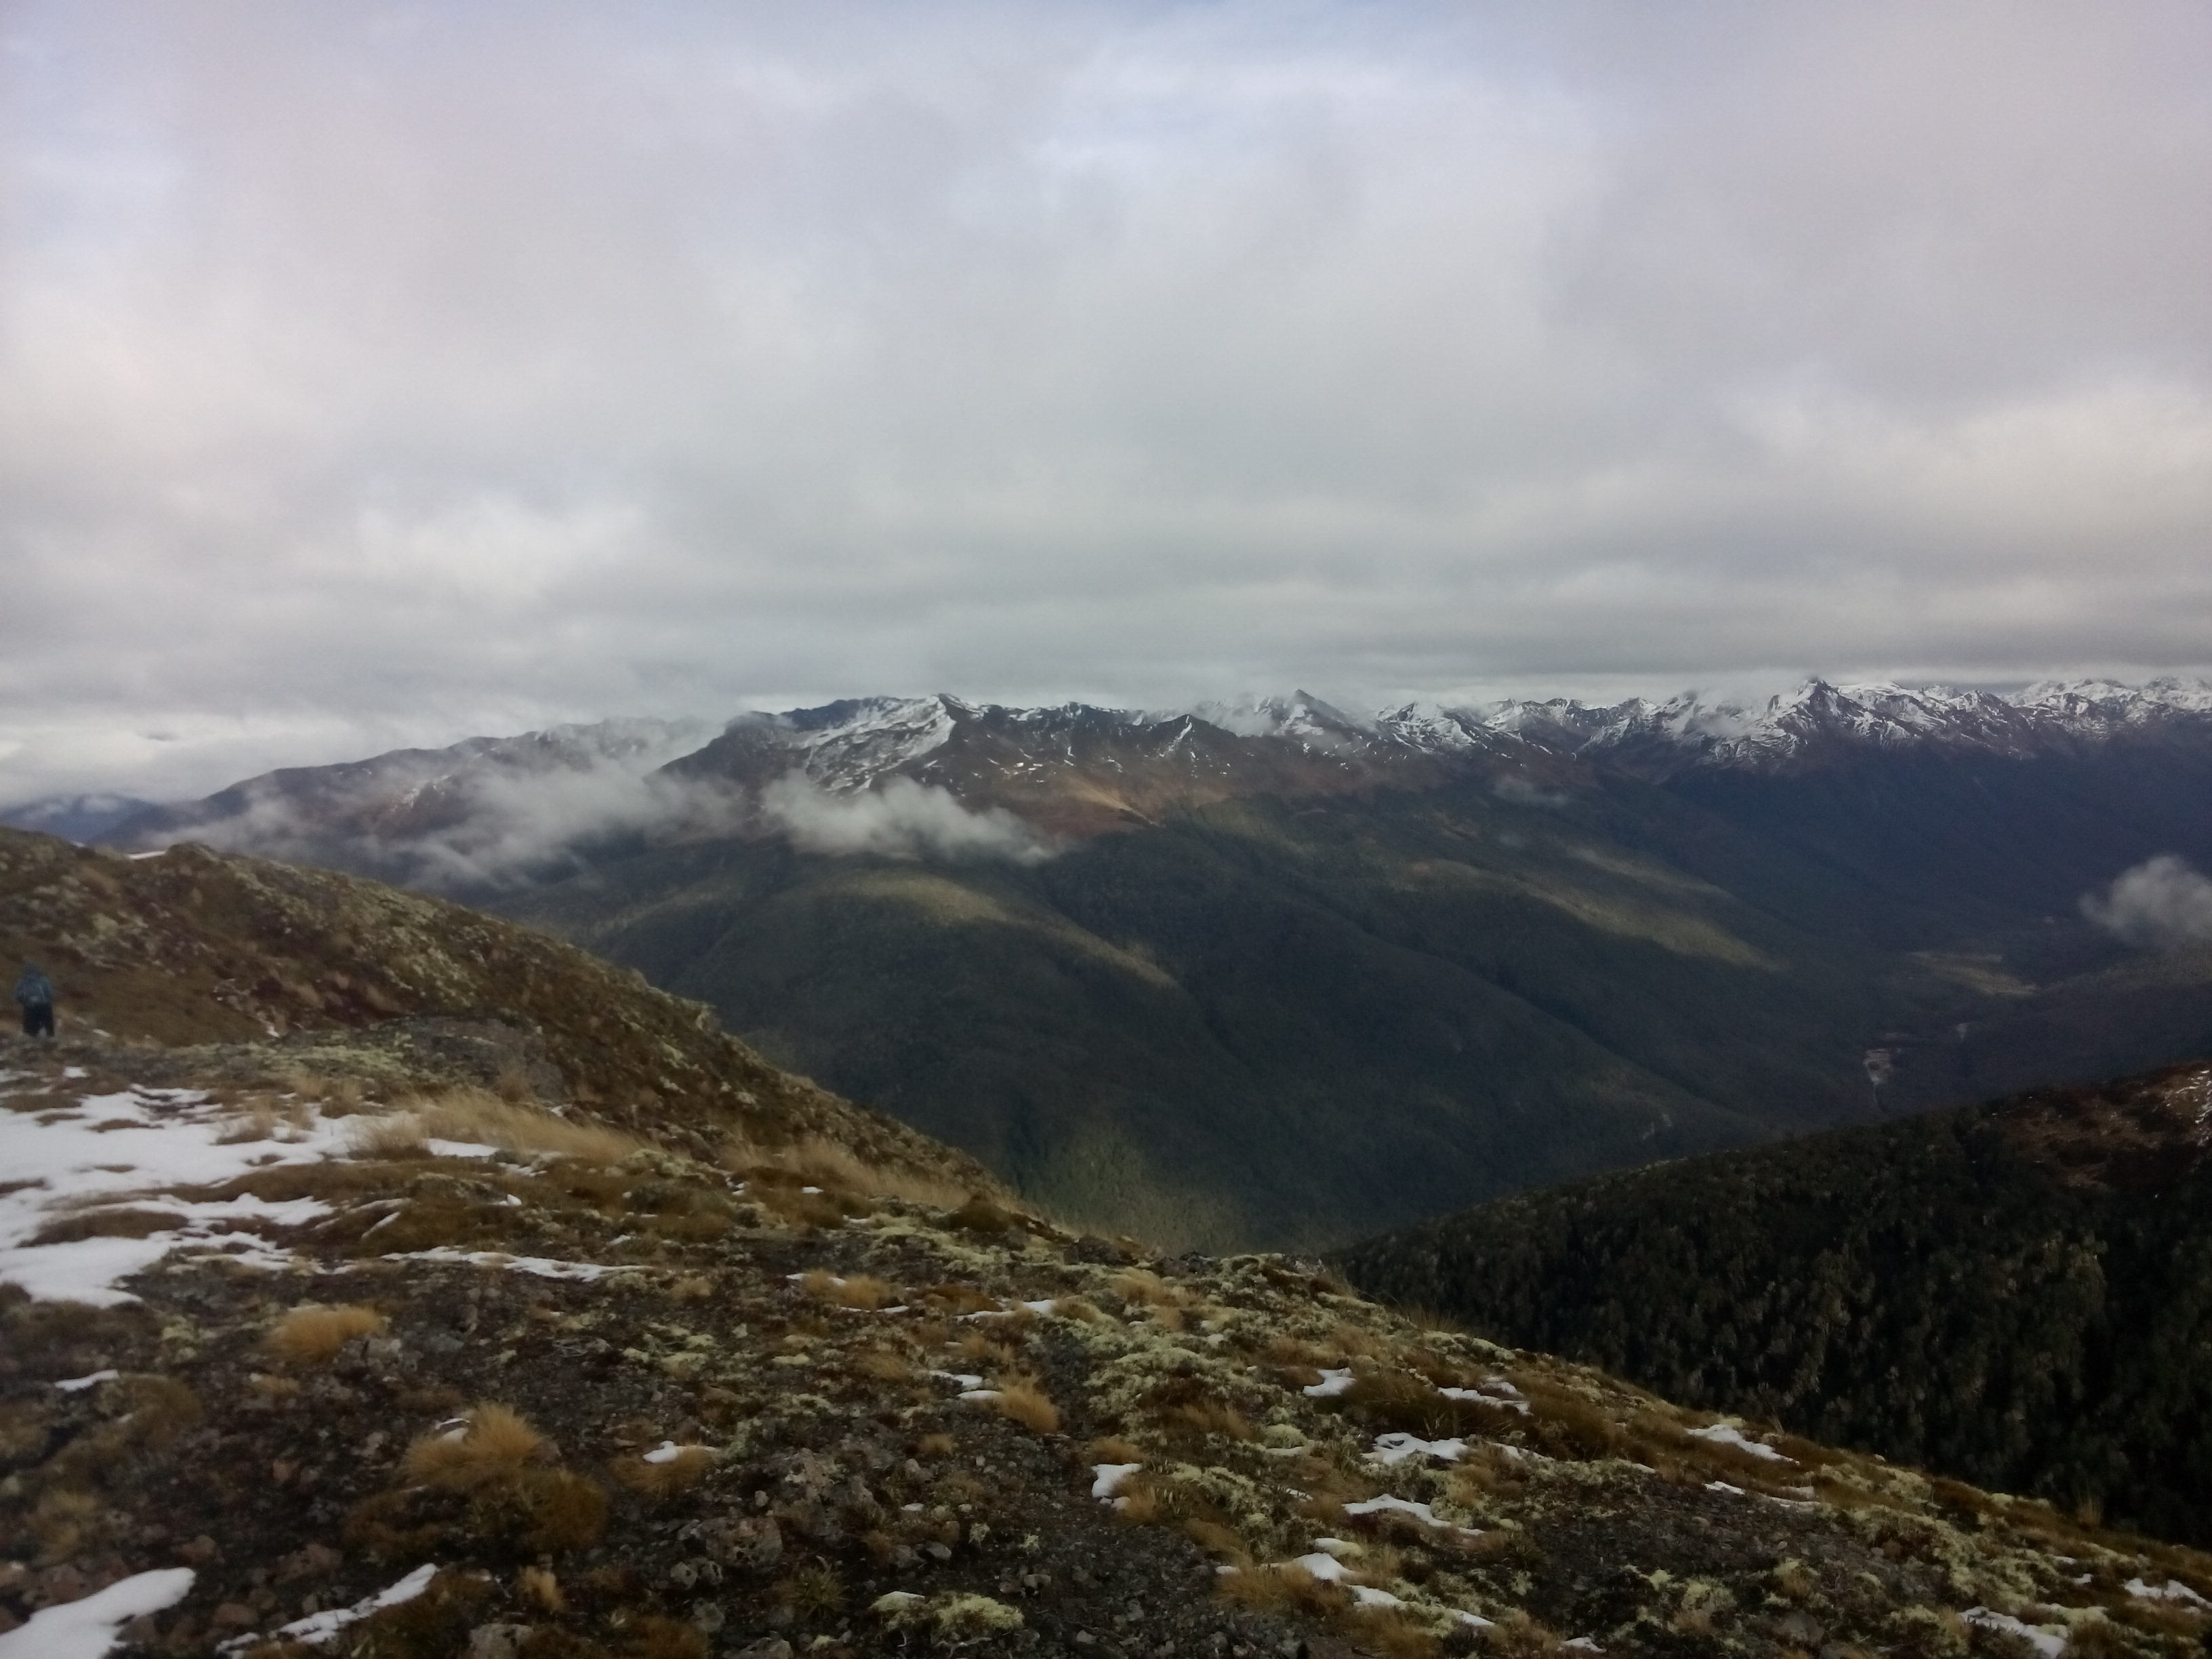
\includegraphics[width=8.5cm]{MtNorma28June2017Photo2}
\end{flushright}
\end{minipage}
\end{figure}

In summer we will attempt to get to the top of Mt Norma, although there was a bit that looked a little tricky.  We shall see.

\begin{flushright}
Robyn, Peter and dog
\end{flushright}

\end{document}
